% id: 0174
% book: RPM 중3-2 수학 · 02 삼각비의 활용
% section: 유형 01 직각삼각형의 변의 길이 구하기
% figure: crop:fig-0174.png
% answer: ①, ②
% answer_source: 답지
% variant_level: 0 (원본 전사)
% 이 파일은 build.mjs 가 items.json 에서 만든다. 고칠 때는 items.json 을 고친다.
\smash{\raisebox{1.5mm}{\dmkichul{대표문제}}}
\noindent\begin{minipage}[t]{0.58\linewidth}\vspace{0pt}\raggedright 오른쪽 그림의 직각삼각형~$\pt{ABC}$에서 $\angle\pt{B}=34^\circ$, $\seg{BC}=x$일 때, 다음 중 $\seg{AB}$의 길이를 나타내는 것을 모두 고르면? \mbox{(정답 2개)}\end{minipage}\hfill\begin{minipage}[t]{0.4\linewidth}\vspace{0pt}\centering \setlength{\dmfigw}{76.8pt}\ifdim\dmfigw>\linewidth\setlength{\dmfigw}{\linewidth}\fi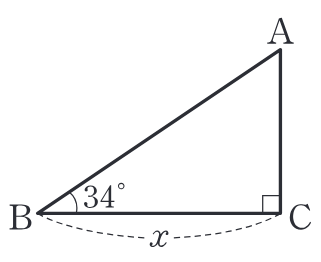
\includegraphics[width=\dmfigw]{figures/fig-0174.png}\end{minipage}\par
\begin{choices32}{\rule[-3ex]{0pt}{8ex}$\dfrac{x}{\sin 56^\circ}$}{\rule[-3ex]{0pt}{8ex}$\dfrac{x}{\cos 34^\circ}$}{\rule[-3ex]{0pt}{8ex}$x\sin 34^\circ$}{\rule[-3ex]{0pt}{8ex}$x\cos 34^\circ$}{\rule[-3ex]{0pt}{8ex}$x\cos 56^\circ$}\end{choices32}
